\documentclass[11pt,letterpaper]{article}
\usepackage[T1]{fontenc}
\usepackage[utf8]{inputenc}
\usepackage{lmodern}
\usepackage{amsmath,amssymb,amsthm,mathtools}
\usepackage[margin=1in]{geometry}
\usepackage{microtype}
\usepackage[dvipsnames]{xcolor}
\usepackage{graphicx,booktabs,array,longtable}
\usepackage{enumitem}
\usepackage{listings}
\usepackage{tikz}
\usetikzlibrary{arrows.meta,positioning}
\usepackage{fancyhdr}
\usepackage{hyperref}
\hypersetup{colorlinks=true,linkcolor=MidnightBlue,citecolor=MidnightBlue,
  urlcolor=MidnightBlue,pdftitle={Simultaneous Tietze Elimination with Shared Circuits},
  pdfauthor={ProveIt research continuation}}
\usepackage[nameinlink,noabbrev]{cleveref}
\setlength{\headheight}{14pt}
\pagestyle{fancy}
\fancyhf{}
\fancyhead[L]{\small ProveIt: Unknot recognition}
\fancyhead[R]{\small Shared singleton eliminations}
\fancyfoot[C]{\thepage}
\setlist{itemsep=3pt,topsep=5pt}
\setlength{\emergencystretch}{2em}
\newtheorem{theorem}{Theorem}[section]
\newtheorem{lemma}[theorem]{Lemma}
\newtheorem{proposition}[theorem]{Proposition}
\newtheorem{corollary}[theorem]{Corollary}
\theoremstyle{definition}
\newtheorem{definition}[theorem]{Definition}
\newtheorem{remark}[theorem]{Remark}
\newcommand{\Z}{\mathbb Z}
\newcommand{\N}{\mathbb N}
\newcommand{\F}{\mathbb F}
\DeclareMathOperator{\supp}{supp}
\DeclareMathOperator{\len}{len}
\DeclareMathOperator{\bits}{bits}
\newcommand{\code}[1]{\texttt{\detokenize{#1}}}
\newcommand{\baselinecommit}{\texttt{483b7397a1086206bc463222094315390c42550d}}
\lstset{basicstyle=\ttfamily\small,breaklines=true,columns=fullflexible,
  keepspaces=true,frame=single,rulecolor=\color{black!18},
  backgroundcolor=\color{black!2},showstringspaces=false,
  xleftmargin=3pt,xrightmargin=3pt,aboveskip=10pt,belowskip=10pt}
\title{\textbf{Simultaneous Tietze Elimination\protect\\with Shared Circuits}\\[5pt]
  \large Linear grammar growth and a certified improvement\protect\\
  to the unknot group stage}
\author{Research continuation for the ProveIt repository}
\date{9 October 2026 (UTC)}
\begin{document}
\maketitle
\begin{abstract}
The current ProveIt recognizer compresses group words and can contract
acyclic forests of two-generator primitive relations. We extend the raw
algebraic operation to arbitrary singleton Tietze relations, including
mixed-sign words with many dependencies. If the chosen dependencies are
acyclic, all selected generators can be eliminated in one shared
straight-line-program compilation. The principal bound is linear in the
number of source grammar nodes, independently of dependency depth and
expanded word length. Its proof uses vertex-disjoint unique-occurrence paths
inside the source grammar. A topologically ordered list of donor slots and
pivots is sufficient for independent checking with constant-size node
summaries.

For an explicit family of validated stabilized unknot diagrams, the pinned
primitive-forest policy takes a linear number of raw batches and normalization
handoffs, and incurs quadratic slot-scanning work. The new operation finishes
in one batch with linear grammar growth and near-linear charged structural
work. We implement source-bound version-eight certificates, independent
compressed and literal replayers, a conservative terminal dispatch rule,
and reproducible comparisons with the complete pinned predecessor.
An eager partial-batch policy exposed a substantial Gordian regression;
the delivered dispatch uses the operation when it can finish at the exact
rank-one endpoint. All remaining relators are checked.

The result is an exact algebraic improvement and a polynomial positive route
on a specified input class. It does not establish a general quasi-polynomial
unknot recognizer. The article distinguishes proved bounds, measured
performance, policy limitations, and the remaining exposure and hierarchy
obligations.
\end{abstract}
\newpage
\begingroup
\small
\tableofcontents
\endgroup
\newpage
\section{Outcome, baseline, and the remaining target}
\label{sec:context}

This continuation gives a larger exact reduction operation for the maintained
unknot recognizer and a concrete asymptotic separation from its preceding
group-stage policy. The new operation eliminates an entire acyclic system of
singleton relations in one shared compilation. It includes relations such as
\[
 c=a b a^{-1},\qquad d=c b^{-1} a c,
\]
which are excluded by a rule restricted to expressing one generator as a
power of one other generator. The expanded replacement words can be very
long. The computation instead preserves their common subexpressions.

The principal mathematical result is an $O(M+r)$ output-grammar bound for a
batch, where $M$ counts the nodes reachable in the original relator grammar
and $r$ is the number of live generators. This bound does not contain the
depth of the dependency graph or the length of the expanded words. The
supporting insight is a disjointness property of the paths to the chosen
singleton occurrences. It bounds the combined cost of extracting all
definitions before the global substitution is performed.

The implementation is accompanied by an independent certificate checker and
measurements against a pinned complete predecessor. It also records a failed
policy experiment. Applying the larger operation at every opportunity can
make subsequent heuristic search substantially worse. The delivered public
option therefore uses a batch when it can finish immediately at an exact
one-generator endpoint; the general algebraic operation remains available
for research and supplied witnesses.

\subsection{What was already present}

The baseline is the public ProveIt repository at commit
\begin{center}\baselinecommit.\end{center}
Its most recent changes in the relevant directory were committed on
9 October 2026 at 01:42:56 UTC.
All predecessor comparisons in this package use that commit, not a small
reimplementation of the old kernel. The inspected files include
\code{compressed_search.py}, \code{compressed_words.py},
\code{primitive_projection.py}, \code{primitive_forest.py}, both source
replayers, the corresponding tests, and the maintained synthesis sections
on primitive projections, forests, and planner accounting
\cite{ProveIt2026}.

The baseline already has several important capabilities. Group words are
stored as exact binary straight-line programs. The search can perform
singleton elimination, Whitehead transformations, and relator operations;
separate source reconstruction replays its certificate. Optional primitive
projections operate on raw words, so expensive normalization can be deferred.
The forest extension permits overlapping primitive donors when each chosen
child is a unit coordinate and their dependencies are acyclic. It shares
parent-power circuits, and the planner caches immutable word summaries while
rebuilding slot and live-generator information for each current state.
These are the starting point of the present work.

The new contribution is therefore not the first use of compression, batching,
or independent replay in this project. It removes the two-generator,
coherent-sign, pure-power restriction from a particular simultaneous
operation and supplies the size argument needed when the definitions are
general words. This comparison concerns exact singleton elimination, the
unpowered case of a primitive donor. The predecessor's separate inference
from proper powers can still use source-established torsion-freeness and
remains available under its existing hypotheses. Previous certificate
formats remain accepted.

\subsection{Claims and their exact scope}

\begin{center}
\small
\begin{tabular}{p{0.29\linewidth}p{0.61\linewidth}}
\toprule
Claim & Scope established in this article \\
\midrule
Exact simultaneous elimination & Any finite group presentation with the
specified raw singleton donors and acyclic dependencies. \\
Linear grammar growth & One shared batch, retaining every other original
relator slot; length metadata still has a nonconstant bit cost. \\
Efficient independent checking & A topologically ordered list of original
donor slots and pivot labels; no replacement-word claims are trusted. \\
Asymptotic stage improvement & An explicit family of validated stabilized
unknot diagrams, relative to the pinned forest policy. \\
Polynomial positive route & Inputs that expose a checked batch to rank one
with zero exponent in every retained relation, after polynomial preparation. \\
General quasi-polynomial recognition & Not established. Global exposure,
representation growth outside this operation, and search costs remain open. \\
\bottomrule
\end{tabular}
\end{center}

The distinction in the last two rows matters. A fast certificate checker
does not imply a fast certificate producer. A fast local reduction does not
bound how long the search takes to reach its hypotheses. An infinite easy
family can demonstrate a strict improvement in the relevant operation
model without establishing a speedup for all difficult unknot diagrams.

\subsection{Relation to the literature}

Shared substitution and compressed free-group algorithms are established
techniques. Schleimer gives a constructive treatment of compressed word
problems and applies shared image descriptions to free-group automorphisms
\cite{Schleimer2008}. Haubold and Lohrey explicitly combine Tietze generator
elimination with straight-line-program substitution and additive local size
growth in their work on compressed HNN-extension problems
\cite{HauboldLohrey2011}. Kapovich's recent Proposition~3.2 gives a quantitative
layered-substitution bound for a specified sequence from a fixed finite
endomorphism family in fixed rank \cite{Kapovich2026}. Those results motivate
the data representation used here. The present proof separately charges
variable-sized donor contexts and variable-rank dependency systems; its
claims do not follow merely by citing a fixed-family substitution theorem.

The group-theoretic equivalence behind a singleton elimination is classical
Tietze elimination. We do not claim that acyclic definitions or that
equivalence are new ideas in combinatorial group theory. The contribution
here is a precise shared-grammar bound, the ordered witness that can be
checked with small summaries, their integration into the current recognizer,
and a reproducible separation from its preceding policy. No exhaustive
priority claim is made for the standalone disjoint-path lemma.

The broader geometric target must also be stated accurately. The 2021
Oxford announcement of Lackenby's work gave $n^{O(\log n)}$, while a 2024
seminar abstract specified $2^{O((\log n)^3)}$; these are distinct bounds
within quasi-polynomial time \cite{Lackenby2021Talk,Lackenby2024Talk}.
The July 2026 preprint develops a hierarchy algorithm and certification
results. Section~9 explicitly leaves several implementation costs
unestimated and bounds iteration count using hierarchy length and surface
pattern-complexity parameters. That preprint does not itself state a
quasi-polynomial running-time theorem \cite{Lackenby2026Hierarchy}. We have not
converted that work into a complete implementation with a proved
quasi-polynomial running time. The group operation in this article is a
separate constructive advance within the existing recognition pipeline.

\subsection{The group endpoint and source provenance}

For a classical knot $K\subset S^3$, its group is infinite cyclic exactly
when $K$ is the unknot; the standard implication uses the foundational
three-manifold results of Papakyriakopoulos \cite{Papakyriakopoulos1957}.
Consequently, if a sound sequence of presentation equivalences leaves one
generator and only zero-exponent relations, it supplies an unknot
certificate. A raw word on one generator need not be the empty string:
$a^t a^{-t}$ is an immediate example. Its exponent can nevertheless be
computed exactly by addition on the compressed grammar.

The public checker reconstructs the presentation from the source planar
diagram and retains every Wirtinger relation, including the redundant one.
It does not accept an arbitrary abstract presentation as a knot certificate.
The local singleton theorem needs no torsion-freeness assumption; the
source binding is still essential for turning its final cyclic-group
conclusion into a topological verdict.

\section{An exact quotient operation for singleton dependency graphs}
\label{alg:setting}

The algebraic operation developed here removes many generators in one
simultaneous substitution. Its donors may involve arbitrarily many other
generators, with repeated letters and mixed signs. The compatibility
condition is an acyclic dependency graph. We first prove the quotient
statement for arbitrary presentations, and then bound the compressed
construction in terms of its actual input grammar. The rank is part of
the input throughout this section.

Let $X$ be the finite set of live generators, with $r=|X|$. Write $F(X)$
for the free group on $X$. A presentation has $m$ retained relator slots
$R_1,\ldots,R_m$, including any empty slots left by earlier operations.
The exact signed words in these slots are represented by roots of one
binary straight-line program $\mathcal G$. Its rules are signed letters,
binary concatenations, and a distinguished empty root. Let $M$ be the
number of nonempty grammar nodes reachable from the current roots.
The words are allowed to contain free cancellation. Their raw spellings,
rather than their reduced lengths, determine the occurrence conditions below.

\begin{definition}[A singleton DAG witness]
\label{alg:def-witness}
A witness chooses a set $C\subseteq X$ of $k$ distinct children and a
distinct donor slot $j(c)$ for each $c\in C$. The raw donor word must have
exactly one occurrence of either sign of $c$, giving a factorization
\[
 D_c:=R_{j(c)}=U_c c^{\epsilon_c}V_c,
 \qquad \epsilon_c\in\{1,-1\}.
\]
Define the right-hand side
\[
 W_c=(V_cU_c)^{-\epsilon_c}.
\]
For each selected child $d$ occurring in $W_c$, put an arrow $c\to d$.
The witness is valid when this graph on $C$ is acyclic. The surviving
generators are $A=X\setminus C$.
\end{definition}

The support of $W_c$ includes every absolute generator label occurring
in it. Signs and multiplicities affect the substituted word but not the
dependency graph. A donor consisting of $c^{\epsilon_c}$ alone is
permitted: its right-hand side is empty and it has no dependencies.
Dependencies on surviving generators also impose no restriction.

Choose a dependency order $c_1,\ldots,c_k$, so that an arrow
$c_i\to c_j$ implies $j<i$. Define words over $A$ recursively by
\[
 I_a=a\quad(a\in A),\qquad
 I_{c_i}=W_{c_i}\bigl[I_h/h:h\in X\bigr].
\]
Only already defined selected images are used in the second formula.
Negative letters receive inverse words, including reversal of their order.
These images define a homomorphism $\Phi:F(X)\to F(A)$.

\begin{theorem}[Simultaneous singleton quotient]
\label{alg:quotient}
For every valid singleton DAG witness,
\[
 \langle X\mid R_1,\ldots,R_m\rangle
 \cong
 \left\langle A\;\middle|\;
   \Phi(R_j),\ j\notin\{j(c):c\in C\}\right\rangle.
\]
Thus all retained roots can be mapped simultaneously, and exactly the
selected donor slots can then be emptied. The assertion holds for every
finitely presented group.
\end{theorem}

\begin{proof}
The equation $U_c c^{\epsilon_c}V_c=1$ is equivalent to
$c=(V_cU_c)^{-\epsilon_c}$; this also holds when either context is empty.
Let $N$ be the normal closure of the selected donors in $F(X)$. Every
donor is killed by $\Phi$, so $\Phi$ induces a homomorphism
$\overline\Phi:F(X)/N\to F(A)$. Inclusion of the surviving generators
induces a homomorphism $\iota:F(A)\to F(X)/N$.

We show in dependency order that $c_i=I_{c_i}$ in $F(X)/N$. The donor
equation gives $c_i=W_{c_i}$ there. Every selected letter in $W_{c_i}$
has an earlier index, so the induction hypothesis replaces it by its
image. This proves the assertion. The two homomorphisms are consequently
inverse on every surviving and selected generator. They are therefore
mutually inverse group homomorphisms. Finally quotient by the images
of all unselected relators. Under this isomorphism those images are
precisely the words $\Phi(R_j)$ stated in the theorem.
\end{proof}

The theorem justifies deletion of a donor even when its mapped raw word
is a nonempty spelling of the identity. No equality query is required for
that deletion. Every other original slot remains present; an unrelated
relator can impose a substantial condition after substitution.

\begin{remark}[Raw occurrences and source hypotheses]
\label{alg:raw-scope}
A signed exponent sum of $1$ or $-1$ does not establish the required
singleton condition: a word may contain a generator twice positively
and once negatively with noncommuting letters between the occurrences.
Conversely, an actual singleton donor needs no torsion-free hypothesis.
The ordinary, exponent-one case of a unit-coordinate power forest is
a special case of this construction. A proper-power donor with several
raw occurrences of its child is not automatically a singleton donor;
the existing root-evidence route remains a separate capability.
If a future extension infers $D_c=1$ from a checked proper-power donor
$D_c^q=1$, $|q|>1$, that inference will require an additional justification,
such as source-established torsion-freeness. It is separate from
Theorem~\ref{alg:quotient}.
\end{remark}

Acyclicity is also substantive. The two donors $ab$ and $ab^{-1}$ allow
the proposed choices $a$ and $b$ individually, but together create a
dependency cycle. Their presentation is $\Z/2\Z$: the first donor gives
$a=b^{-1}$ and the second gives $b^2=1$. Deleting both generators and
both donors would instead give the trivial group. An individual
singleton test therefore cannot replace the compatibility check.

\section{Linear grammar growth through shared contexts}
\label{alg:compression}

Compressed substitution is a well-established method in algorithmic
group theory; see Schleimer~\cite{Schleimer2008}. For fixed rank and a
fixed finite family of endomorphisms, Kapovich's quantitative layered
substitution statement constructs an SLP of size $O(M+t+1)$ for a
specified length-$t$ composition, with constants depending on that rank
and family~\cite[Proposition~3.2]{Kapovich2026}. Here the rank and the
donor words vary with the input. The following argument controls the
extraction and composition of these variable-sized definitions directly
from their shared source grammar.

\subsection{The disjointness of the selected occurrence paths}

For a selected child $c$, follow its unique occurrence from the donor
root through the binary grammar. At each concatenation, exactly one
child word contains $c$. This gives a path $H_c$ ending at a signed
terminal of $c$. The grammar can share that terminal and many other
nodes with other words; the path is defined by the occurrence in this
particular donor.

\begin{lemma}[Disjoint hole paths]
\label{alg:hole-paths}
For distinct selected children $c,d$, the paths $H_c$ and $H_d$ have
no grammar node in common. In particular,
\[
 \sum_{c\in C}|H_c|\le M.
\]
\end{lemma}

\begin{proof}
A node on $H_c$ expands to a word containing $c$. Since the donor
contains $c$ only once, every concatenation on the path has only one
child containing it, and a node containing $c$ cannot occur twice in
the donor's unfolded derivation. The path is thus well defined even
in a heavily shared grammar.

Suppose a node belonged to both $H_c$ and $H_d$. Its expansion would
contain both selected children. It occurs within $D_c$, so deleting
the unique occurrence of $c$ from that donor leaves an occurrence of
$d$. Hence $W_c$ contains $d$. The same reasoning within $D_d$ shows
that $W_d$ contains $c$. This creates the two-cycle $c\to d\to c$,
contradicting the witness condition. The paths are disjoint, and each
is a subset of the $M$ reachable source nodes, proving the sum bound.
\end{proof}

The lemma does not say that whole donor grammars are disjoint. Large
subwords over shared parents or survivors can occur in many donors.
It controls precisely the paths on which cutting out the chosen
occurrences requires new grammar structure. This distinction removes
the otherwise unnecessary factor of $k$ from a bound obtained by
charging a full grammar-height traversal independently to every donor.

\begin{lemma}[All contexts from one source grammar]
\label{alg:contexts}
The words $V_cU_c$, for all selected children, can be represented using
the source nodes and at most $M$ additional binary concatenation nodes.
Their construction has $O(M+k)$ grammar events and uses no reduction,
equality test, or expanded-word allocation.
\end{lemma}

\begin{proof}
Descend $H_c$ while accumulating its prefix and suffix. When the path
enters a right child, append the left sibling to the prefix. When it
enters a left child, prepend the right sibling to the suffix. Siblings
are reused by node reference. Their order is the order they have in
the original word, so the final contexts are exactly $U_c$ and $V_c$.
Each internal path node calls at most one context concatenation.
One final concatenation joins the suffix to the prefix.

There is one terminal node on each $H_c$. Thus the number of possible
new context nodes, including the final joins, is at most
\[
 \sum_{c\in C}(|H_c|-1)+k
 =\sum_{c\in C}|H_c|\le M.
\]
Empty contexts and interning can reduce this number.

The independent implementation obtains the two contexts by the exact
slices $[0,p)$ and $[p+1,|D_c|)$, where $p$ is the unique occurrence
position. Both boundary traversals follow $H_c$. At a path node, only
one of the two complementary slices can need a new concatenation:
which one depends on which child contains the hole. Fully included
sibling subwords are reused. The same bound therefore applies to this
alternative construction.
\end{proof}

\subsection{Compiling both orientations of every needed word}

Let $\mathcal H$ be the union of the source grammar and the context
nodes from Lemma~\ref{alg:contexts}. It has at most $2M$ nodes. For
each node $v$ use two virtual states $(v,+1)$ and $(v,-1)$, representing
its final substituted word and the inverse of that word. If $v=uv'$,
the positive state depends, in order, on $(u,+1),(v',+1)$; the negative
state depends on $(v',-1),(u,-1)$. An unselected terminal produces
itself or its inverse.

A terminal $c^\delta$ with $c\in C$ is redirected to the context
$V_cU_c$. In orientation $\sigma$, its context orientation is
$-\epsilon_c\delta\sigma$. This one sign formula handles both donor
signs, both occurrences of the generator in other words, and both
virtual orientations. It also avoids constructing and traversing a
separate inverse grammar for each already composed image.

\begin{lemma}[Acyclic signed compilation]
\label{alg:signed}
The augmented virtual graph is acyclic. Evaluating each needed virtual
state once produces the images $I_c^{\pm1}$ and all required mapped
relators with at most $4M$ reachable nonempty output grammar nodes.
\end{lemma}

\begin{proof}
Before terminal redirects, the graph follows source and context
concatenations and is acyclic. A directed cycle introduced by the
redirects must pass through selected terminals. Between two successive
selected-terminal redirects, a path starts in a defining context for
some child $c$ and reaches an occurrence of another selected child $d$.
Such a segment witnesses the dependency $c\to d$. A virtual cycle
would therefore give a directed closed walk, and hence a directed
cycle, in the dependency graph. The stipulated acyclicity excludes it.

Evaluate virtual states in a topological traversal. A terminal needs
at most one letter node, a concatenation at most one concatenation
node, and a redirect only an alias to its already evaluated state.
The defining equations and the sign convention show inductively that
these values are the desired substituted words. There are at most
$2|\mathcal H|\le4M$ virtual states. Each output node is the value of
one of these states, proving the node bound. States shared by several
images or relators are evaluated only once.
\end{proof}

All definitions are included among the traversal goals, even if no
unselected relator uses their children. This prevents a checker from
ignoring an invalid but unused part of a proposed schedule. Only after
the complete construction succeeds are the retained root array and
the live-generator set replaced. A failed resource check can leave
newly allocated arena nodes, while the represented presentation
remains the original one.

\begin{theorem}[Uniform size bound]
\label{alg:linear-size}
All node counts in this statement exclude the distinguished empty node.
A valid singleton DAG batch on a shared reachable source grammar of
$M$ nodes has a compressed output with at most $4M$ nonempty grammar
nodes and the original $m$ root slots. A persistent arena can perform
the construction by adding at most $5M$ nodes to its previous allocated
count. In particular, when no unreachable nodes were previously
allocated, its total allocated count is at most $6M$.
\end{theorem}

\begin{proof}
At most $M$ context nodes are allocated, followed by at most $4M$
nodes from signed compilation. The source nodes already existed.
Lemma~\ref{alg:signed} bounds the reachable output independently of
the source and temporary context nodes retained by the arena.
Previously allocated unreachable nodes are unchanged and must be
added to the total when applying an arena-wide memory cap.
\end{proof}

The constants are conservative; cached letters, empty contexts and
interning often reuse nodes. The substantive property is their
independence of dependency depth, rank, expanded donor lengths, and
the number of occurrences of a parent in another child's definition.

\section{An ordered certificate with small summaries}
\label{alg:ordered}

The version-eight move records an ordered list of pairs consisting of
an original donor slot and a chosen child. No substituted words,
occurrence positions, supports, or grammar node identifiers are trusted
as certificate data. The order itself is a topological witness.

Give every survivor rank zero and the $i$th chosen child rank $i$.
For every source node $v$, compute $q(v)$, the largest selected rank
in its expansion, and $t(v)$, its occurrence count capped at two.
The empty root has summary $(0,0)$ and a terminal of rank $h$ has
summary $(h,1)$. At a concatenation $v=uv'$, put
\[
 q(v)=\max\{q(u),q(v')\},
\]
\[
 t(v)=\min\!\left\{2,
 t(u)\mathbf 1_{q(u)=q(v)}+
 t(v')\mathbf 1_{q(v')=q(v)}\right\}.
\]
Counts at rank zero need not distinguish the surviving generators:
every selected donor must have a positive maximum rank.

\begin{proposition}[Verification by ranked maxima]
\label{alg:ranked-max}
An ordered list with distinct children and distinct donor slots is a
valid singleton DAG witness in the supplied order if and only if the
donor of its $i$th child has summary $(i,1)$.
Every valid singleton DAG admits an order satisfying these conditions.
\end{proposition}

\begin{proof}
The recurrence computes the maximum rank and the capped multiplicity
of that rank by induction over the source grammar. Only the $i$th
selected child has rank $i$. Summary $(i,1)$ says that this child occurs
exactly once and no later child occurs in its donor. Removing its
occurrence leaves only survivors and earlier children, so every
dependency is earlier. Conversely, those two occurrence conditions
immediately imply summary $(i,1)$. Finally every finite acyclic graph
has a dependency order, to which the equivalence applies.
\end{proof}

Each summary has constant cardinality and $O(\log(r+1))$ bits. The
check avoids storing an $r$-bit support mask at every grammar node.
The same maxima locate each unique occurrence: on its hole path,
exactly one child has the donor's maximum rank. The contexts can
therefore be independently sliced without an expanded occurrence scan.

The checker first verifies the record types, live generator membership,
slot ranges and distinctness conditions, and checks that source terminals
use live labels. It then checks each donor's ranked maximum against the
intact current roots before constructing that donor's contexts. No
presentation mutation is committed until every donor and the full
composition have passed. Boolean values are not accepted as integer
identifiers. All other relator slots are mapped and retained. These
checks connect the combinatorial witness to the
exact quotient theorem; a source-bound public verdict must additionally
reconstruct the diagram and replay the complete preceding proof prefix.

The producer uses a simpler order already present in the input: numeric
generator order. It caches, for each immutable node, its maximum
absolute label and that label's count capped at two. The first current
slot whose maximum occurs once supplies that maximum's donor. Chosen
children are then sorted increasingly. All their dependencies are
smaller, so the result is valid. Cached content summaries never cache
slot positions or a previous live-generator set; those are reconstructed
for each current presentation.

This numeric policy is incomplete. Let an anchor $a$ have a larger
numeric label than every leaf $c_i$, and take donors $a^q c_i$ with
$q\ge2$. Their maxima repeat, so the producer finds no pivot. Selecting
every $c_i$ is nevertheless a valid batch with a common surviving
anchor. A suitable order places the anchor first and exposes all
these donors. The general ordered checker accepts that witness.
Thus a restriction in discovery does not become a restriction on the
mathematical class of certificates it can verify.

\section{Encoding, bit operations, and phase composition}
\label{alg:complexity}

Put $N=M+r+m$, and let $\ell$ bound the bit length of generator labels.
After reindexing the reachable grammar, pointer fields require
$O(\log(N+2))$ bits. The output grammar, live-generator description and
retained root list consequently have canonical encoded length
\[
 O\!\left(N\bigl(\log(N+2)+\ell\bigr)\right).
\]
This bound describes the word representation itself. Cached arithmetic
metadata in an implementation can be larger.

In particular, a binary grammar with $Q$ nonempty nodes represents no
word longer than $2^Q$. Induction in topological order proves this:
a terminal has length one and each concatenation adds two lengths
of earlier nodes. The output word-length integers therefore have
$O(M+1)$ bits by Theorem~\ref{alg:linear-size}. The source, context and
compiled nodes involved in this batch can therefore require $O(M^2)$
bits of cached length metadata. Any metadata belonging to previously
allocated unreachable nodes is additional unchanged storage. Construction
operates on these integers; it does not pay for their represented
word lengths. For a retained root list $\mathcal R$, define
\[
 B(\mathcal R)=\max\!\left\{1,
   \left\lceil\log_2\!\left(1+
     \max\bigl(\{\len(R):R\in\mathcal R\}\cup\{0\}\bigr)
   \right)\right\rceil\right\}.
\]
Let $B_{\mathrm{in}}$ and $B_{\mathrm{out}}$ denote this quantity before
and after the batch, respectively, using the exact raw word lengths.
A separate elementary bound is
\[
 B_{\mathrm{out}}\le (k+1)B_{\mathrm{in}}+O(k+1),
\]
To see this, put $L=\max(1,\max_j\len(R_j))$ for the original roots.
Every defining word has at most $L$ letters. Defining the images in
dependency order multiplies the largest image length by at most $L$
at each step, and mapping an original root introduces one further
factor of at most $L$. The final root length is at most $L^{k+1}$.
The direct grammar bound is frequently sharper and suffices for
polynomial bit complexity.

Ranked summary evaluation, context extraction and signed compilation
have $O(N)$ grammar or slot events. Sorting the producer's $k$ selected
labels adds $O(k\log(k+1))$ comparisons; the maintained work counter
charges this sorting explicitly. Thus linear grammar growth does not
mean exactly linear producer work. Graph indexing and the source
postorder also have their ordinary implementation costs. A deterministic
implementation can use comparison-based indexing, and a Python
implementation uses its usual dictionary behavior.

The verifier's rank summaries have $O(\log(r+1))$ bits; the producer's
numeric-label maxima have $O(\ell)$ bits. Generator comparisons have
$O(\ell)$-bit operands, and position or length additions have
$O(M+1)$-bit operands. The number of these operations is polynomial
in $N$. This gives a deterministic polynomial bit bound in the encoded
input parameters, with an absolute degree independent of the rank
and DAG depth. Under the straightforward arithmetic representation,
the possible quadratic total cost of length additions is already a
conservative polynomial allowance. The abstract work counter is a
cooperative resource measure, rather than a claim to count those bit
operations exactly.

An internal application helper also accepts unsorted acyclic schedules
through a general dependency-mask fallback. Its polynomial mask cost
is separate from the public ordered-certificate route. Similarly,
literal replay pays for actual expanded output and can exhaust its
allocation allowance on a batch whose compressed construction is small.

\begin{theorem}[Composition of raw singleton batches]
\label{alg:phases}
Suppose $d$ successive operations consist solely of valid singleton DAG
contractions. If the initial encoded parameters, including any retained
arena storage, are polynomially bounded by $N_0$, the total construction
and ordered-verification cost
has a bound
\[
 \operatorname{poly}(N_0)\,2^{O(d)}.
\]
The constants do not depend on the ranks or dependency depths of
the individual batches.
\end{theorem}

\begin{proof}
Each contraction multiplies the reachable grammar bound by at most an
absolute constant, and a persistent arena obeys the conservative
recurrence $A_{i+1}\le6A_i$ for its nonempty allocated node count. Rank never
increases and the number of retained slots is fixed. Hence all grammar
and metadata parameters after $i$ phases are bounded by a polynomial
in $N_0$ times $6^{O(i)}$. Substitute this into the fixed polynomial
per-phase bound and sum over $i\le d$. The resulting geometric bound
has the stated form.
\end{proof}

From polynomial-size diagram data, $d=O(\log n)$ such phases would
have polynomial total raw-contraction cost; a polylogarithmic bound
on $d$ would give a quasipolynomial bound. The theorem does not bound
the discovery of useful new donors, the normalization work between
contractions, or the length of a search using other operations.
It is a local composition statement. For example, a later raw
singleton need not occur in its original slot: from slots $xg$ and
$x$, eliminating $x$ using the first exposes $g$ in the second.
Simply collecting the original slot--child pairs does not fuse that
history into one initial witness.

\section{The difficulty of choosing the largest batch}
\label{alg:selection}

Efficient verification of a supplied schedule leaves a separate
optimization problem. The following elementary reduction identifies
a concrete limit on exact unrestricted batch selection. Its source
is the classical independent-set problem, equivalently the complement
of vertex cover in the standard NP-completeness framework
of Karp~\cite{Karp1972}.

\begin{definition}[Singleton DAG selection]
\label{alg:selection-problem}
Given a finite list of explicit relator words and an integer $b$, ask
whether there is a valid singleton DAG witness selecting at least
$b$ distinct children. Both the donor assignment and a valid order
may be chosen. The compressed variant supplies the words by an SLP.
\end{definition}

\begin{theorem}[Selection is NP-complete]
\label{alg:selection-hardness}
Singleton DAG selection is NP-complete. NP-hardness already holds for
explicit positive words in which each relator has exactly one
singleton generator. Thus it also holds when the candidate child of
each donor is fixed in advance.
\end{theorem}

\begin{proof}
A certificate consists of the chosen distinct slots and children in
dependency order. Its size is polynomial in the input. Direct
occurrence and order checks verify it for explicit words; the ranked
summary verifier does so for compressed words. Both decision problems
therefore belong to NP.

For hardness, let $H=(V,E)$ be a finite simple undirected graph. Use
one generator $x_v$ for each vertex and one relator
\[
 D_v=x_v\prod_{u\in N_H(v)}x_u^2
 \qquad(v\in V),
\]
where each neighborhood is written in any fixed order. The total
explicit length is $|V|+4|E|$. The generator $x_v$ occurs once in
$D_v$, whereas every other generator present occurs twice. Thus
$x_v$ is the only possible singleton child for that donor.

A chosen set of donors corresponds to a vertex set $S\subseteq V$.
For adjacent selected vertices $u,v$, donor $D_u$ contains $x_v$ and
donor $D_v$ contains $x_u$. Their dependency graph contains the
two-cycle $x_u\to x_v\to x_u$. Therefore every valid selected set
is independent in $H$. Conversely, if $S$ is independent, none of
its selected donors contains another selected child. All its other
letters are survivors, so its dependency graph has no edges and is
valid. The largest possible batch has size exactly $\alpha(H)$.
Using the same threshold $b$ gives a polynomial reduction from
independent set and proves the claim.
\end{proof}

The reduction concerns arbitrary current-word presentations. It does
not establish hardness for Wirtinger presentations, for states known
to arise from a validated knot, or for the numeric-order planner.
Nor does it imply that finding a useful smaller batch is difficult
on a particular geometric family. It explains why maximum-cardinality
selection should be a distinct research objective rather than an
unproved property of a greedy scan.

\subsection{The recognition scope of a terminal batch}

If a checked batch leaves one generator $a$ and every retained mapped
relator has exponent sum zero at $a$, the resulting presentation is
$\langle a\mid\varnothing\rangle\cong\Z$. At rank one, exponent
sum completely determines a group word. At larger rank the same
test is insufficient: a commutator has zero exponent vector and can
still impose a nontrivial relation.

For a source-established knot group, the standard cyclic-group
characterization of the unknot supplies the final topological
conclusion. The construction theorem makes this a polynomial
positive route whenever the required source preparation and prefix
replay also have polynomial bounds. It supplies no claim that every
unknot reaches such a state efficiently.

The final public search policy invokes the operation only when it
finds at least two pivots and exactly $r-1$ selected children. Otherwise
the current presentation and the legacy operation order remain
unchanged. This terminal guard separates the valid general algebraic
operator from a policy for applying partial batches during heuristic
search. An algebraic quotient preserves the group while potentially
changing later normalization costs and search choices.

Relative to the same compressed search with its other options held
fixed, the guard gives logical preservation of positive successes
when resources are uncapped: it either reaches a checked rank-one
terminal or continues through the old presentation states. This
comparison does not identify the compressed search with the public
API's default explicit backend; enabling the option also selects
compressed search. Planning overhead still consumes real time and the shared
work allowance, so the assertion is not fixed-budget performance
dominance. The general all-DAG quotient and verifier remain useful
for future policies whose exposure and downstream progress can be
analyzed separately.

\section{A strict improvement on an actual diagram family}
\label{sec:family}

\subsection{The source diagrams and their presentations}

For $r\geq 2$, take the closure of the $(r+1)$-strand braid
\[
 B_r=\sigma_1\sigma_2\cdots\sigma_r.
\]
This is an unknot: repeatedly remove the last positive Markov stabilization,
ending at the one-strand trivial braid. It has $r$ crossings in the supplied
diagram. The repository constructs the diagram using
\code{Diagram.from_braid(r+1, list(range(1,r+1)))}. Its diagram validation
and presentation reconstruction are included in the experiments.

With the baseline's arc labels and free and cyclic reduction of the initial short
Wirtinger words, its presentation has $r$ live generators and the following
$r$ retained slots:
\begin{align}
 R_1&=x_1x_2^{-1},\label{eq:chain-first}\\
 R_i&=x_1x_i x_1^{-1}x_{i+1}^{-1},
       &&2\leq i\leq r-1,\label{eq:chain-middle}\\
 R_r&=x_r x_1^{-1}.\label{eq:chain-last}
\end{align}
The final slot is retained throughout the experiment. All three size
parameters---crossing number, initial live rank, and slot count---are $r$.
The number of braid strands is $r+1$; confusing it with the group rank gives
off-by-one errors in the batch counts.

\subsection{The new batch}

Choose $x_{i+1}$ as the pivot of $R_i$, for $1\leq i<r$. Each is its donor's
largest label and occurs once. The selected definitions are
\begin{equation}
 I_2=x_1,\qquad I_{i+1}=x_1 I_i x_1^{-1}\quad(2\leq i<r).
 \label{eq:chain-images}
\end{equation}
Every dependency is earlier in the displayed order. The $r-1$ pivots
therefore form one valid batch. For $i\geq2$, the exact raw spelling of the
image is
\begin{equation}
 I_i=x_1^{i-1}x_1^{-(i-2)},\qquad
 |I_i|=2i-3,\qquad \operatorname{exp}_{x_1}(I_i)=1.
 \label{eq:chain-raw}
\end{equation}
These expressions are deliberately not freely reduced. The shared grammar
stores each $I_i$ through the previous image, using a bounded number of
concatenation nodes per step. Its size is $O(r)$ even if both orientations
are prepared for reuse.

The only unselected slot becomes $I_r x_1^{-1}$, whose exponent is zero.
The exact one-generator check therefore finishes the certificate. For
$r\geq3$, the delivered two-pivot threshold permits this one-batch route.
The $r=2$ case can use the existing rank-two endpoint and is immaterial to
the asymptotic separation.

\begin{figure}[htbp]
\centering
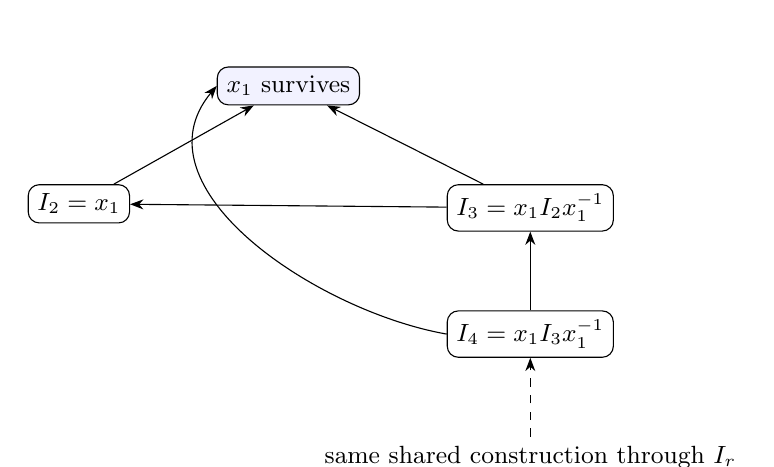
\begin{tikzpicture}[node distance=10mm and 11mm,>=Stealth,
  every node/.style={font=\small}]
\node[draw,rounded corners,fill=blue!5] (root) {$x_1$ survives};
\node[draw,rounded corners,below left=of root] (a) {$I_2=x_1$};
\node[draw,rounded corners,below right=of root] (b) {$I_3=x_1 I_2 x_1^{-1}$};
\node[draw,rounded corners,below=of b] (c) {$I_4=x_1 I_3 x_1^{-1}$};
\node[below=of c] (d) {same shared construction through $I_r$};
\draw[->] (a)--(root);
\draw[->] (b)--(a);
\draw[->] (b)--(root);
\draw[->] (c)--(b);
\draw[->] (c.west) to[out=170,in=230] (root.west);
\draw[->,dashed] (d)--(c);
\end{tikzpicture}
\caption{A definition depends on earlier images and the surviving generator.
Arrows describe dependence, not a sequence of separate presentation rewrites.
The entire system is evaluated in one shared traversal.}
\label{fig:chain-sharing}
\end{figure}

\subsection{What the pinned forest policy must do}

\begin{proposition}[Exact phase count for the pinned family policy]
\label{prop:family-phases}
On the presentation \eqref{eq:chain-first}--\eqref{eq:chain-last}, the pinned
\code{primitive_forest=True} search with its rank-two endpoint enabled uses
\[
 \left\lfloor\frac{r-1}{2}\right\rfloor
 \quad\text{forest batches},\qquad
 \left\lfloor\frac{r-2}{2}\right\rfloor
 \quad\text{normalization handoffs}.
\]
For $r\geq3$, the singleton batch uses one raw batch and no normalization
handoff.
\end{proposition}

\begin{proof}
Only the two end relations initially have coherent signs on two generators.
Every middle relation contains both signs of $x_1$ and is excluded by the
baseline's primitive candidate descriptor. Its forest selects the two end
donors, eliminating $x_2$ and $x_r$ as $x_1$. The newly exposed end words
are still mixed-sign raw words until the explicit normalization step.
The complete normalization handoff reduces them to the end relations of
the same chain with two fewer live generators. Interior words keep the
same form, up to the surviving labels, while the original slot array
retains its length $r$.

This establishes an induction reducing live rank by two per forest batch.
An even initial rank finishes after the last handoff at the old rank-two
endpoint. An odd initial rank reaches three live generators, contracts
both remaining children, and finishes with the raw rank-one exponent
check without another handoff. The formulas follow, including the base
case $r=2$. The new construction was established in
\eqref{eq:chain-images}--\eqref{eq:chain-raw}.
\end{proof}

\begin{corollary}[A structural work separation]
\label{cor:family-work}
The pinned forest policy performs $\Omega(r^2)$ charged abstract work on
this group-stage family. The delivered singleton route has $O(r)$ grammar
nodes and $O(r\log(r+1))$ charged structural work, including the explicit
charge for sorting its certificate pivots.
\end{corollary}

\begin{proof}
The predecessor retains all $r$ slots and scans them in each of
$\Theta(r)$ phases. Each scan is charged, giving the lower bound without
making any assumption about the cost of its additional normalization work.
The new source, context, and signed image grammars all have $O(r)$ nodes.
Maximum-and-count summaries and endpoint exponents are computed once per
relevant node or slot. The implementation additionally sorts the $r-1$
pivots and charges $O(r\log(r+1))$ work for that operation.
\end{proof}

This is a statement about the supplied presentation and the pinned policy.
It is not a lower bound for all ways to recognize these diagrams. In
particular, earlier diagram simplification often removes their crossings
quickly. Group-stage measurements deliberately invoke the checked group
routine on the intact source so that this operation is actually exercised.
Complete-recognition measurements keep the earlier stages enabled and are
reported separately.

\subsection{An exponential raw-word stress family}

The implementation tests also use noncoherent recursive definitions whose
unreduced images double in length at each level. The 512-generator case
retains a raw word of length $2^{511}$ while using a small grammar.
Expansion, inversion by a separate whole-image traversal, free reduction,
cyclic reduction, and compressed equality are disabled during the batch in
this test. This checks the resource mechanism that the proof requires.

This second family is an abstract algebraic stress test. Its expanded length
is an exact integer derived from the recurrence, not a number of letters
actually allocated. It is not presented as a difficult knot corpus or a
wall-time comparison against a program asked to allocate $2^{511}$ letters.

\section{Implementation, evidence format, and conservative dispatch}
\label{sec:implementation}

\subsection{The implemented operation}

The new producer is \code{fastunknot/singleton_dag.py}. Its planner stores
one immutable pair per grammar node: the maximum absolute generator label
and that label's occurrence count, capped at two. Concatenation retains the
larger maximum, or adds the capped counts when the maxima agree. Each
current root is inspected in its original slot; the first eligible donor
for each child is chosen. The output is sorted by child label, making its
dependency order explicit.

The cache contains word content only. Relator slots and current live-label
membership are checked afresh. This matters because roots can move between
slots, normalization creates different roots, and a previously live
generator can have been eliminated. Planning neither mutates the
presentation nor allocates substituted images.

Application builds the prefix and suffix surrounding each unique pivot.
The inverse required by a positive pivot is represented by a virtual sign.
A single iterative traversal then evaluates signed grammar states, with
selected terminals redirecting to their definitions. An inverse
concatenation reverses the order of its children. Each signed state is
evaluated at most once. Both images of a definition are shared when needed;
they are not independently expanded or repeatedly inverted.

The helper also supports arbitrary internally supplied acyclic schedules.
An ordered schedule uses rank maxima and capped counts, regardless of its
numeric labels. An out-of-order internal schedule can use a generic
presence/repetition mask fallback and a cycle check. That fallback has a
larger polynomial metadata cost. The public certificate path always uses
an ordered witness and needs no dense support masks.

\subsection{Version-eight certificates}

A batch move contains only its kind and an ordered pivot list:
\begin{lstlisting}
{
  "kind": "singleton_dag",
  "pivots": [
    {"relation": 0, "generator": 2},
    {"relation": 1, "generator": 3}
  ]
}
\end{lstlisting}
The order is part of the evidence. All selected generators in a donor's
right-hand side must occur earlier in this list. Surviving generators have
rank zero. The certificate gives no replacement word, inferred exponent,
dependency list, source grammar node identifier, or claimed hash equality
for the checker to trust.

The complete group certificate still binds the input planar diagram,
method, status, moves, and terminal evidence. A trace using this move has
version eight. Both source replayers reject it if relabelled as an older
format. Previously supported versions remain accepted through their
existing interpretation.

\subsection{Independent compressed and literal replay}

The new checker module, \code{singleton_dag_verify.py}, imports no producer
helper. It requires exact field sets, actual integers rather than boolean
substitutes, valid original slots, live pivot labels, distinct slots, and
distinct pivots. It independently assigns certificate ranks and verifies
that each donor has its own pivot as a unique maximum-rank occurrence.
This checks singleton status and dependency order in one pass.

Its compressed implementation locates the pivot position, obtains the two
source substrings, and builds its own signed substitution evaluation.
Its context construction differs from the producer's direct sibling
accumulation. The literal implementation instead extracts explicit words,
builds and checks the dependencies, and substitutes definitions in
topological order with allocation checks before growth. The latter is an
independent oracle for bounded-size examples, not a polynomial method in
compressed input size when the expanded output is enormous.

Every definition is checked even when all its occurrences would lie in
discarded donor slots. This prevents an unused cyclic system from escaping
validation. Both replayers retain all non-donor slots. Rejection leaves
the root array and live-generator set unchanged; a compressed arena may
have allocated temporary nodes before rejection or resource exhaustion.
No claim of rollback of internal cache allocation is needed for soundness.

The outer checker independently reconstructs all source Wirtinger relations
before reading the moves. It finishes a rank-one trace only after checking
every retained root's exponent. Cyclicity is not inferred from one selected
relation or from the number of remaining labels alone.

\subsection{Why the delivered dispatcher is terminal-only}

The first integration applied every discovered batch of at least two
pivots. That policy was algebraically sound and worked on many actual
diagrams. It also changed the residual spelling on the Gordian fixture
enough to make the subsequent heuristic search hit a large work cap.
The local node bound does not control the difficulty of later Whitehead
or relator operations on that residual state.

The delivered public option therefore applies a batch only if
\begin{equation}
 2\leq |C|=|X|-1.
 \label{eq:terminal-guard}
\end{equation}
If the guard fails, planning has not changed the relators, their slots,
the live labels, or the established move order of the same compressed
backend with the same other flags. Search continues from the
intact state. If it succeeds, the batch leads directly to the existing
exact rank-one exponent check. The general batch operation and its proof
remain useful to research clients; the dispatcher makes a narrower choice
about when to use it during heuristic search.

This guard has a simple logical property. For a source knot presentation
and an uncapped correct preceding trace, an exact elimination to rank one
must have zero exponent in every retained relation: otherwise the resulting
one-generator presentation would have finite abelianization, contradicting
the knot group's abelianization $\Z$. The checker still verifies the
exponents explicitly. The public option can thus finish at the guarded
state without requiring any subsequent search heuristic to be effective.

Planning consumes resources even when it skips a batch. Therefore the
unchanged-state property does not imply identical completion under every
finite work or time allowance. The feature stays opt-in, and the experiments
record capped nondecisions and overhead. No universal wall-time dominance
over the predecessor is claimed.

\subsection{Public entry points and compatibility}

The group-stage interfaces accept \code{singleton_dag=True}; this selects
compressed search and independent compressed replay. The whole recognizer
accepts \code{group_singleton_dag=True} together with \code{use_group=True}.
The command line exposes \code{--group-singleton-dag}, which enables the
group stage automatically. For example:
\begin{lstlisting}[language=Python]
from fastunknot import Diagram
from fastunknot.group_certificate import group_decide

d = Diagram.from_braid(129, list(range(1, 129)))
result = group_decide(d, singleton_dag=True, seconds=None)
assert result["status"] == "UNKNOT"
assert result["certificate"]["version"] == 8
\end{lstlisting}

The option defaults to false. Existing projection and forest flags retain
their original meaning. Source replay accepts old certificates, and an audit
compares all three old modes against the entire pinned package. The Rust
port is not changed in this package. The new Python implementation uses the
standard library and requires the same Python language baseline as the
maintained package.

\subsection{Resource model}

The same work, node, initial-letter, and caller-cancellation mechanisms as
the surrounding compressed search remain in force. The new operation
does not use expanded word length as a loop bound. Its counters separately
report planner attempts, new immutable descriptors, candidate slots,
unique-occurrence path steps, signed evaluation states, batch pivots,
newly allocated nodes, and skipped partial batches.

The existing \code{projection_normalizations} counter counts raw-to-normal
handoffs in the common search loop. A terminal singleton batch causes none.
In the retained eager prototype, handoffs after a partial singleton batch
use that existing counter name; the result files preserve the original
names rather than silently recategorizing them.

Charged work is an implementation accounting measure. It includes explicit
charges such as the pivot sort and is useful for diagnosing scaling, but
it is neither a hardware instruction count nor a substitute for the
separate bit-complexity proof and completed-call timings.

\section{Source audit and controlled measurements}
\label{sec:experiments}

The experiments support two different conclusions. The new operation gives
a substantial checked group-stage improvement on the explicit source family
of Section~\ref{sec:family}. It does not improve the total running time of the
preserved ordinary corpus. We retain both findings, the unsuccessful eager
policy, and every recorded bounded nondecision. The proofs establish the
asymptotic statements; finite timing measurements test the implementation
and the mechanism responsible for its observed behavior.

\subsection{Independent package isolation and timing boundary}

The comparison imports the complete Python package from the pinned commit
and the complete modified package in separate persistent worker processes.
Both are imported under their normal name, \code{fastunknot}. This matters
because some maintained modules use absolute imports: loading two versions
under aliases inside one Python process can accidentally mix their
dependencies and invalidate a comparison. Frozen package trees are included
in the archive. Every Python source file, and the measurement harness itself,
is hashed before and after a run. Those hashes are identical across the
final guarded audit and both timing experiments.

The worker measures exactly
\begin{lstlisting}[language=Python]
start = time.perf_counter()
result = fn(Diagram.from_pd(pd), **options)
elapsed = time.perf_counter() - start
\end{lstlisting}
where \code{fn} is \code{group_decide} for the stage experiment and
\code{recognize} for the ordinary corpus. The interval includes fresh source
validation and the complete call, including mandatory independent compressed
source replay whenever a group certificate is produced. Package import,
transport between processes, traversal of
the returned evidence, and JSON serialization are outside the interval.
The timing is therefore a completed checked call, not just a favorable
inner kernel.

Each input has six arms: predecessor default, predecessor forest, delivered
singleton, and an identical A/A repeat of each. Each arm has one excluded
warmup. Five subsequent rounds are retained; the six arms are randomly
shuffled within each round using a fixed recorded seed. The workers use
\code{PYTHONHASHSEED=0}. The environment was Python 3.12.14 on
Linux 6.18.44, x86-64, glibc 2.39. The precise inputs, options, sample orders,
statuses, counters, proof objects, and hashes are in the result JSON files.

Tables report the median elapsed time of each named arm. A displayed
comparison ratio is the median of the five within-round time ratios;
it is not the ratio of the two displayed medians. A ratio above one favors
the singleton arm. A/A controls reveal ordinary timing variation, especially
on submillisecond cases. This is a single-environment experiment with five
measured rounds, not a statistical confidence interval or evidence of a
universal wall-time improvement.

\subsection{Source-bound audit and regression coverage}

The guarded audit contains 81 validated source cases, comprising 75 distinct
planar-diagram arrays: the preserved
19-case corpus, fixed-seed valid one-component braid closures, and seven
stabilized circles. For each source, it compares the predecessor and current
implementation with all new options disabled, with primitive projection,
and with primitive forest. All 243 comparisons agree exactly in the returned
certificates or bounded nondecisions. Their recorded statistics also agree.
This comparison uses the whole pinned package and checks compatibility
of the existing modes, rather than comparing against a reimplemented model.

With the singleton option enabled, 54 sources yield positive certificates.
All 54 pass both the literal and the compressed independent source replayers.
There are no newly closed and no lost positive cases relative to either
predecessor default or predecessor forest in this finite audit. Of the 54
proofs, 29 use version eight, 22 use version five, and three use version one.
The version-eight proofs contain 29 batches and 307 certified pivots.
An unsuccessful attempt is not counted as a successful certified batch.

The maintained test suite discovers and runs 1,008 tests successfully, with
zero failures, errors, or skips. This is the pinned suite plus 16 new test
methods. The authoritative ledger records the completed count, source hashes,
Python version, and empty failure and error lists. Historical reference
modules imported by older tests are included with the reproduction snapshot.

The new methods contain 80 randomized metadata cases and 100 randomized
signed DAG cases, including orders that disagree with numeric label order.
They compare every retained relator with literal substitution, test actual
stabilized diagrams through 128 crossings, exercise huge shared powers and
the $2^{511}$ raw-length family, and check resource exhaustion and caller
cancellation. Adversarial cases include duplicate slots, duplicate pivots,
boolean identifiers, fabricated singleton conditions, dependency cycles,
old-version relabelling, and an obstructing residual relation that must be retained.
Selected tests disable producer helpers, normalization, or expansion during
compressed replay to check the intended independence and raw boundary.

A separate small exhaustive review enumerates 3,698 ordered local cases over
three generators. Exactly 360 are accepted and 3,338 rejected, with exact
agreement between the independently computed criterion and both replayers.
Accepted outputs agree as raw words; rejected inputs retain their roots and
live sets. This review also checks that a skipped partial probe preserves a
raw forest state and its subsequent normalization handoff. These tests
provide concrete evidence for the implementation. They do not replace the
algebraic proof or establish recognition completeness.

\subsection{Checked group stage on the stabilized-circle family}

The parameter $n$ in Tables~\ref{tab:stage-times} and
\ref{tab:stage-structure} is the crossing count, the initial presentation
rank, and one less than the number of braid strands. Earlier diagram
simplification is deliberately bypassed. These diagrams are easy unknots
obtained by stabilization, and the stage experiment isolates the group
operation analyzed above.

All 150 measured calls and 30 excluded warmups complete. The common stage
options are \code{seconds=None}, a work allowance of 50,000,000, a node
allowance of 1,000,000, and compressed search. Every arm includes independent
compressed source replay before its timer stops.

\begin{table}[tbp]
\centering
% Generated by experiments/summarize_singleton_dag.py; do not hand edit.
% Fresh source checked group stage only; five paired rounds; ratios are medians of ratios.
\begingroup
\small\setlength{\tabcolsep}{4pt}
\begin{tabular}{rrrrrr}
\toprule
$n$ & Default ms & Forest ms & Singleton ms & Default/singleton & Forest/singleton \\
\midrule
16 & 6.217 & 3.552 & 1.352 & 4.203 & 2.401 \\
32 & 15.764 & 7.348 & 2.859 & 5.755 & 2.570 \\
64 & 60.712 & 18.818 & 5.372 & 12.112 & 3.813 \\
128 & 219.120 & 60.203 & 10.477 & 21.205 & 5.656 \\
256 & 876.726 & 244.618 & 23.583 & 36.468 & 9.444 \\
\bottomrule
\end{tabular}
\endgroup

\caption{Completed checked group-stage calls on stabilized circles. Times
are medians in milliseconds; the last two columns are medians of paired
ratios. The singleton column uses the delivered terminal guard.}
\label{tab:stage-times}
\end{table}

\begin{figure}[tbp]
\centering
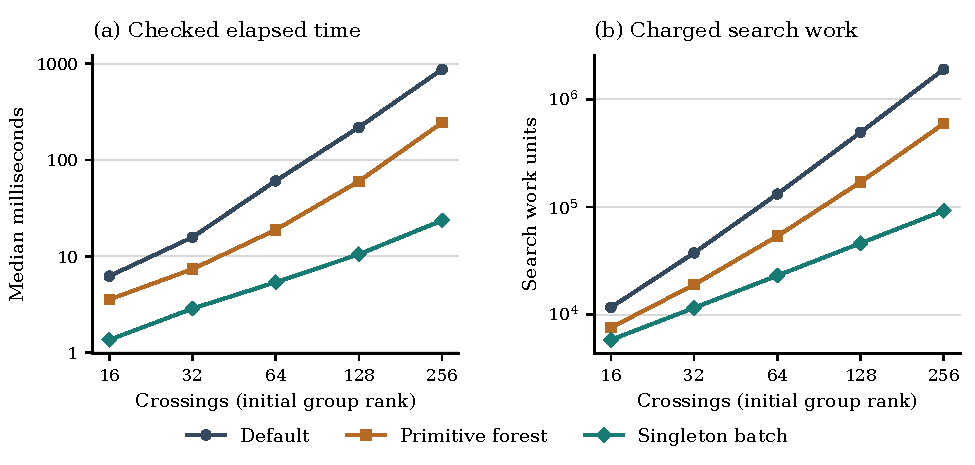
\includegraphics[width=\linewidth]{figures/stage_scaling.pdf}
\caption{Measured group-stage elapsed time and charged search work on the
same sources. Points are observed values; connecting segments aid reading
and are not fitted asymptotic laws. Earlier diagram simplification is
bypassed. The mathematical operation-count separation is proved separately.}
\label{fig:stage-scaling}
\end{figure}

At $n=256$, the median elapsed times are 876.7 ms for default, 244.6 ms for
forest, and 23.58 ms for singleton. The paired median improvements are
36.47 and 9.44, respectively. The large change is consistent with replacing
127 forest batches and 127 normalization handoffs by one batch containing
255 pivots. The corresponding work counters are 1,905,056, 595,473, and
92,547.

\begin{table}[tbp]
\centering
% Generated by experiments/summarize_singleton_dag.py; do not hand edit.
% One singleton batch in every row; nodes are search-arena total nodes.
\begingroup
\small\setlength{\tabcolsep}{4pt}
\begin{tabular}{rrrrrr}
\toprule
$n$ & Forest batches & Singleton pivots & Default nodes & Forest nodes & Singleton nodes \\
\midrule
16 & 7 & 15 & 419 & 121 & 147 \\
32 & 15 & 31 & 1611 & 249 & 307 \\
64 & 31 & 63 & 6299 & 505 & 627 \\
128 & 63 & 127 & 24891 & 1017 & 1267 \\
256 & 127 & 255 & 98939 & 2041 & 2547 \\
\bottomrule
\end{tabular}
\endgroup

\caption{Structural counters for the stage experiment. Every singleton
row uses one batch. Node counts are total allocated search-arena nodes,
including persistent nodes, rather than only reachable output nodes.}
\label{tab:stage-structure}
\end{table}

Singleton does not minimize every size measure. At 256 crossings the
forest arena has 2,041 nodes, while singleton has 2,547. The default has
98,939. The canonical JSON certificates occupy 49,244 bytes for forest,
12,770 for singleton, and 17,600 for default. The observed improvement
comes from avoiding repeated passes and normalization, not from a claim
that its arena is always smaller than the forest arena. The explicit
linear node formulas on this family and the general upper bound have
different meanings from finite elapsed times.

Across the stage cases, the paired A/A median ratios range from 0.901 to
1.104. This is enough variation to discourage fine interpretation of
small differences, while being far smaller than the large stage ratios
at the upper sizes. No speedup for the complete recognizer on this easy
family is inferred: an earlier simplifier can already close it.

\subsection{Ordinary whole-recognizer workload}

The ordinary experiment preserves all 19 cases and their original source
diagrams. It performs 570 measured calls and 114 excluded warmups, all of
which complete. The options include the group stage and relator operations,
compressed search, a group work allowance of 20,000,000, a group time
allowance of 10 seconds, an overall allowance of 12 seconds, and 50,000
objects. No incomplete call is silently dropped from a ratio.

Fifteen unknots reach the checked group stage. The trefoil and figure-eight
finish earlier through the homogeneous Seifert-genus filter; Conway and
Kinoshita--Terasaka finish through the modular Jones filter. Differences in
the times of these four early-closing knots cannot be attributed to a
singleton operation that was never reached.

\begin{table}[tbp]
\centering
% Generated by experiments/summarize_singleton_dag.py; do not hand edit.
% U_G: unknot via group stage; K_S: knotted via homogeneous Seifert genus; K_J: knotted via Jones. Only Gordian has a singleton batch.
\begingroup
\small\setlength{\tabcolsep}{4pt}
\begin{tabular}{llrrrr}
\toprule
Input & Outcome & Default ms & Forest ms & Singleton ms & Default/singleton \\
\midrule
survivor-00 & $\mathrm{U}_{G}$ & 12.022 & 13.303 & 11.997 & 0.970 \\
survivor-01 & $\mathrm{U}_{G}$ & 11.000 & 10.582 & 10.389 & 1.059 \\
survivor-02 & $\mathrm{U}_{G}$ & 12.929 & 11.724 & 11.987 & 0.943 \\
survivor-03 & $\mathrm{U}_{G}$ & 8.406 & 9.513 & 8.876 & 0.848 \\
mirror-03 & $\mathrm{U}_{G}$ & 23.508 & 24.634 & 18.523 & 1.245 \\
survivor-04 & $\mathrm{U}_{G}$ & 7.378 & 8.019 & 7.540 & 0.911 \\
survivor-05 & $\mathrm{U}_{G}$ & 18.598 & 19.196 & 15.077 & 1.234 \\
survivor-06 & $\mathrm{U}_{G}$ & 7.467 & 7.769 & 8.048 & 0.925 \\
survivor-07 & $\mathrm{U}_{G}$ & 14.327 & 15.372 & 20.256 & 0.747 \\
survivor-08 & $\mathrm{U}_{G}$ & 4.836 & 7.888 & 5.384 & 0.956 \\
mirror-08 & $\mathrm{U}_{G}$ & 13.089 & 14.260 & 15.950 & 0.807 \\
survivor-09 & $\mathrm{U}_{G}$ & 5.324 & 5.786 & 7.994 & 0.669 \\
survivor-10 & $\mathrm{U}_{G}$ & 4.759 & 4.740 & 5.076 & 0.889 \\
survivor-11 & $\mathrm{U}_{G}$ & 4.995 & 5.103 & 5.676 & 0.879 \\
gordian & $\mathrm{U}_{G}$ & 952.834 & 993.982 & 1005.899 & 0.950 \\
trefoil & $\mathrm{K}_{S}$ & 0.039 & 0.059 & 0.049 & 0.779 \\
figure-eight & $\mathrm{K}_{S}$ & 0.042 & 0.041 & 0.047 & 0.880 \\
conway & $\mathrm{K}_{J}$ & 0.637 & 0.622 & 0.655 & 0.952 \\
Kinoshita--Terasaka & $\mathrm{K}_{J}$ & 0.589 & 0.632 & 0.672 & 0.919 \\
\bottomrule
\end{tabular}
\endgroup

\caption{Completed whole-recognizer calls on the preserved ordinary corpus.
$\mathrm U_G$ means an unknot closed through the group stage;
$\mathrm K_S$ and $\mathrm K_J$ are knots closed by the Seifert-genus and
Jones filters. Times are median milliseconds, and the final column is the
paired median ratio. Only Gordian actually uses a singleton batch.}
\label{tab:ordinary}
\end{table}

Under the terminal guard, only Gordian uses the new operation. The other
fourteen unknots keep the default version-five proof while paying for
eligibility planning. Their individual timing variations are not evidence
that singleton contraction accelerated their search. Per-case A/A medians
span 0.896--1.249, including the very short cases.

For each measured round, sum the elapsed times over the complete 19-case
workload before forming a ratio. The medians of those five paired workload
ratios are
\[
 \frac{T_{\rm default}}{T_{\rm singleton}}=0.954856,
 \qquad
 \frac{T_{\rm forest}}{T_{\rm singleton}}=0.985518.
\]
Both favor the predecessor, with a modest overall difference. The analogous
workload A/A medians are 0.977439 for default, 0.986358 for forest, and
1.001674 for singleton. This is a workload-weighted aggregate, not a
typical-case estimate: Gordian accounts for about 86\% of total elapsed
time in each policy. Its medians
are 952.8, 994.0, and 1,005.9 ms in the same order. This record supports
keeping the feature opt-in and improving the cost of eligibility discovery.
It provides no ordinary-corpus acceleration or expanded recognition coverage.

\subsection{The failed eager policy and the delivered guard}

The earlier eager implementation applied a discovered batch whenever it
contained at least two pivots, even when many generators remained. Its
81-source audit yielded 53 positive certificates, no new positive, and
one lost positive: the 141-crossing Gordian fixture. The initial partial
batch eliminated 60 generators. Subsequent search on the changed residual
presentation exhausted the work allowance of 20,000,000 without producing
a certificate. The complete eager snapshot and audit are retained, so
the correction can be assessed against the actual counterexample.

The final guarded search skips 125 partial candidates on Gordian and later
uses a terminal batch of three pivots. Its version-eight certificate is
9,621 bytes. Its search work is 1,292,253, compared with 1,215,145 and a
9,663-byte proof for predecessor default. Thus the guard restores the
source-checked result in this experiment while adding some work. The 60
eager attempted pivots are reported as an unsuccessful experiment, not
added to the count of certified pivots.

The issue was downstream search behavior, not a failure of the exact
quotient theorem. The example makes a useful methodological point for
future work: a locally cheaper and algebraically sound transformation
can worsen a bounded heuristic. Productive exposure, residual-state
quality, and resource-aware scheduling need evidence and bounds of their
own. The terminal guard is a narrowly justified way to use the proved
operation while that research remains open.

\section{Consequences for the quasi-polynomial programme}
\label{sec:research}

\subsection{What obstacle has been removed}

The new bound removes dependency depth from the cost of one prescribed
singleton system. A chain of a thousand definitions need not cause a
thousand complete rewrites of the relator grammar. All definitions and
their inverses can be composed together with a constant-factor bound on
the grammar size. The preserved dependency structure also admits a short
ordered witness whose validity can be checked without first constructing
all substituted words separately.

This improves the situation at a concrete point in the project. The old
forest policy was already capable of sharing long powers, but mixed signs
and additional dependencies excluded middle relations on a simple actual
diagram family. The new operation exposes those relations immediately and
avoids the resulting linear chain of scans and normalization handoffs.
The certified group-stage measurements agree with that explanation.

The eager-policy regression shows a different obstacle. A smaller
description after an exact quotient need not be a better input to an
existing heuristic. Search quality depends on which relations remain
visible, which letters are repeated, and what subsequent transformations
become cheap. Grammar size, the number of live generators, expanded length,
and the cost of later search are different quantities. The final terminal
guard avoids needing to predict the latter for this release.

\subsection{A useful amortized planning bound}

The delivered terminal probe can run at many search states without using
the general batch at any of them. Its additional discovery cost is therefore
worth accounting for separately.

\begin{proposition}[Cached planning across a trace]
\label{prop:amortized-planning}
Suppose a search trace invokes the singleton planner $h$ times, retains
$m$ relator slots, and never has more than $r_0$ live generators. Let $Q$
be the number of distinct arena nodes whose immutable maximum-and-count
summary is first encountered across these invocations. The planner's
charged structural work is
\[
 O\!\left(Q+h\bigl(m+r_0\log(r_0+1)+1\bigr)\right),
\]
apart from the ordinary bit cost of keys and label comparisons.
\end{proposition}

\begin{proof}
Each immutable node's summary is constructed once. Its binary children
give only a bounded number of stack events, so all fresh metadata costs
$O(Q)$. A root already in the cache stops its descent immediately.
Current slots, candidate membership, and distinct-child selection cost
$O(m+r_0)$ per invocation. The selected list has at most $r_0$ entries;
the explicit sorting allowance costs $O(r_0\log(r_0+1))$.
Summing over the invocations gives the bound.
\end{proof}

This result avoids an unnecessary factor $hM$ for repeatedly rescanning
unchanged shared subgrammars. It does not bound $Q$ or $h$ for the complete
recognizer. Whitehead moves, overlap operations, and normalization can
create additional nodes and additional states; their costs remain part of
the larger research problem. It also explains why an exact early probe can
still add a modest measured overhead when it seldom fires.

\subsection{What a general quasi-polynomial theorem still requires}

For the algebraic route, a complete proof needs a quantitative exposure
result: every unknot in the chosen input model must reach a useful terminal
or another complete decision method after controlled preparation. Such a
result would have to bound the number of states visited, the size of their
shared representations, the work of normalization and relator discovery,
and certificate replay. Efficient primitives establish none of these
global existence and scheduling statements by themselves.

The raw phase theorem in Section~\ref{alg:complexity} can be used once its
hypotheses are actually supplied. In particular, $d=O((\log n)^2)$ pure
singleton phases from polynomial-size data yield an
$n^{O(\log n)}$ raw-contraction bound. With $d=O(\log n)$ they yield a
polynomial raw-contraction bound. Interleaved normalization or unrelated
moves require their own bounds; they cannot be placed inside the same
constant-factor recurrence without proof. The delivered guarded search
uses at most one singleton batch in a completed certificate, but may
perform many preceding search steps.

For the geometric route suggested by Lackenby's programme, the key
obligations remain constructive surface selection, encoded cutting and
attachment data, effective parallelity-bundle operations, controlled
hierarchy depth, and the total bit cost of all intermediate objects
\cite{Lackenby2026Hierarchy}. Agol--Hass--Thurston orbit counting is a
foundational example of obtaining polynomial work in a compressed normal
surface description without expanding its pieces \cite{AgolHassThurston2006}.
Lackenby's fast curve algorithms offer related boundary-surface primitives
\cite{Lackenby2026Curves}. These results are relevant tools, but they do
not imply that the missing hierarchy can be selected within the target
budget. This article does not identify its presentation DAG with a
three-manifold hierarchy.

\subsection{Further questions with concrete success criteria}

\paragraph{1. Better orders with bounded discovery cost.}
The fixed numeric order misses valid batches, even on relabelled stars.
Can one compute a small deterministic portfolio of orders that exposes
substantially more terminal batches on actual Wirtinger states? A useful
result would combine a restricted structural theorem with complete-call
measurements that charge every unsuccessful order. The NP-completeness
result for unrestricted positive presentations rules out treating maximum
batch selection as an automatically easy preprocessing problem. It does
not rule out efficient algorithms for the planar source class or useful
parameterized algorithms.

\paragraph{2. A structural characterization of terminal exposure.}
Which knot diagrams have a Wirtinger presentation admitting a singleton
DAG to one surviving generator, before any further word transformation?
Existence is invariant under a pure generator renaming, because the witness
can be transported with its order; the numeric planner's success need not
be invariant. How does exposure change under a different presentation
construction or Reidemeister simplification? A characterization should
distinguish existence of a witness from success of one chosen order. It should
also specify whether the input is the raw four-letter presentation or
the initially freely and cyclically reduced version.

\paragraph{3. Quantitative exposure after controlled transformations.}
Can a diagram class broader than descending or visibly stabilized unknots
be shown to reach a terminal singleton system after polynomial or
polylogarithmically many bounded transformations? The desired theorem
must charge the construction of those transformations, not merely show
that some sequence exists. This would be a direct route from the local
result to a stronger restricted recognition theorem.

\paragraph{4. Partial batches with a proved handoff guarantee.}
The Gordian experiment supplies a concrete rejection test for future
partial-batch policies. A replacement policy should retain the positive
coverage and compare the whole checked stage with the guarded version.
Mathematically, seek a potential that controls both representation size
and the next search operation, or a reversible scheduling scheme that
preserves the intact predecessor state with a proved total-cost bound.
Simply choosing the largest available batch is not justified by the
present experiments.

\paragraph{5. Raw closure with persistent substitutions.}
Can several raw singleton phases be represented with an additive
description bound rather than the conservative constant-factor recurrence?
The tempting proof by unioning original donor-pivot pairs is invalid:
after eliminating $x$ using $xg$, the original slot $x$ exposes the newly
introduced singleton $g$. A successful construction must track that
provenance, empty images, and newly exposed occurrences. It should also
bound the discovery cost of the closure itself.

\paragraph{6. Memory reclamation consistent with source replay.}
The current arena retains nodes that become unreachable. The theorem
bounds new allocations relative to the reachable source, and explicitly
adds pre-existing unreachable storage. Can old nodes be compacted with a
verified remapping that preserves caches, certificate provenance, and
the cost of subsequent comparisons? A useful implementation should report
live nodes, allocated nodes, auxiliary metadata bits, and wall time
separately.

\paragraph{7. General primitive and proper-power donors.}
The new operation is strongest when the donor itself has a literal
singleton. Existing primitive-power certificates can infer additional
definitions under source-established torsion-freeness. Can a larger
mixed batch combine these two kinds of evidence while preserving linear
context construction and independent replay? Non-unit rank-two primitive
relations and cyclic dependency components require their own quotient
analysis; they cannot simply be admitted as additional DAG edges.

\paragraph{8. Endpoints with a small remaining rank.}
Rank one has a particularly cheap and complete exponent criterion.
For higher rank, identify restricted residual presentations admitting
equally explicit complete checks, then allow a batch only when it reaches
one of those checked endpoints. A theorem parameterized by the actual
residual structure would be more informative than one parameterized only
by the number of remaining generator names.

\paragraph{9. Certificates as separate reusable mathematical objects.}
The ordered witness describes a presentation equivalence independently of
the search that found it. A Lean formalization of the quotient theorem,
the ranked-summary checker, and the signed grammar evaluator would make
that separation precise. It would still need an independent account of
diagram-to-presentation reconstruction and the classical topological
endpoint before becoming a formal unknot recognizer.

\paragraph{10. Representative benchmarks and crossover prediction.}
The actual source-family speedups are large, whereas the ordinary corpus
shows overhead. A next benchmark should contain more diagrams that survive
the early filters, preserve source and verdict provenance, and compare
features under both generous and production resource allowances. Prediction
of when to invoke the terminal probe should be assessed using withheld
cases. Measurements should retain all nondecisions and A/A controls and
should distinguish a faster group stage from a faster complete recognizer.

\subsection{Recommended next research priority}

The most direct next mathematical target is a restricted exposure theorem
coupled to a small order portfolio. It would address a condition that the
current implementation can already exploit and check. The most direct
engineering target is a cheap, evidence-based invocation policy for the
guarded terminal probe. Both can use the delivered corpus, the eager
Gordian counterexample, and the independent checker as fixed evaluation
tools. A general quasi-polynomial claim should wait for the corresponding
global size and work bounds.

\appendix
\section{Integration and reproducibility}
\label{app:reproduction}

\subsection{Archive contents and source identity}

The archive is a self-contained research and integration bundle. Its
\code{article/} directory contains this PDF, the complete modular \LaTeX{}
source, bibliography, generated tables, and vector and raster figures.
\code{integration.patch} applies the implementation and its new tests to
the pinned repository. The matching \code{repo_overlay/} contains only
new or changed files, so it can be reviewed without extracting an entire
second repository over a working checkout.

The runnable final snapshot is at
\begin{lstlisting}
snapshots/final/Topology/UnknotRecognition/fast/
\end{lstlisting}
It contains the complete Python package, maintained tests, and required
fixtures. The neighboring \code{reports/} subdirectories contain historical
reference implementations imported by those tests. The archive omits the
unrelated large \code{fast/results/} collection and generated Python bytecode.
It includes complete predecessor and eager-prototype Python package snapshots
at \code{snapshots/baseline/} and \code{snapshots/eager/} for isolated comparison.
The final snapshot has the exact source bytes used by the guarded records.

The \code{experiments/} directory contains the independent worker harness,
summary and figure generators, completed test ledger, exhaustive local
review, and four principal records:
\begin{center}
\small
\begin{tabular}{lp{0.57\linewidth}}
\toprule
Record & Evidence retained \\
\midrule
\code{audit-guarded.json} & Source cases, all legacy comparisons, independent
replay outcomes, positive certificates, and bounded nondecisions. \\
\code{stages-guarded.json} & Full completed-call timings and structural
counters on the five stabilized-circle sizes. \\
\code{benchmark-guarded.json} & Every round and A/A arm for all 19 ordinary
whole-recognizer cases. \\
\code{audit-eager.json} & The rejected partial-batch policy, including the
Gordian work-limit regression. \\
\bottomrule
\end{tabular}
\end{center}

The original ordinary-corpus record is retained byte-for-byte as
\code{experiments/corpus.json}. Its SHA-256 is
\begin{lstlisting}
ed7ae3116c89a294e0bcf716cf027f4c80b6bcf48523e6a0bb0e4ecb97d7e89b
\end{lstlisting}
It comes from report 46's cyclic-overlap research overlay at the pinned
commit. The harness reads its source diagrams and expected verdicts; it
does not import that report's algorithms to obtain the new results.

The manifest records the pinned commit, file hashes, snapshot roles, and
verification results. Checksums identify source and evidence bytes; they
are provenance aids, not a replacement for mathematical or source replay
verification. The included verification script checks the manifest,
snapshot-to-experiment identities, and the exact corpus and harness hashes.

\subsection{Applying the implementation}

From a clean ProveIt checkout at the pinned commit, inspect and apply the
patch using the archive's absolute path:
\begin{lstlisting}[language=bash]
git apply --check /path/to/unknot_singleton_dag_20261009/integration.patch
git apply /path/to/unknot_singleton_dag_20261009/integration.patch
\end{lstlisting}
The delivered patch changes five existing Python modules, adds the
producer and independent verifier, adds two test modules, and documents
the option in \code{SINGLETON_DAG.md}. The patch does not modify the Rust
implementation. An integration onto a later commit requires a normal
review of intervening changes; a successful application against the pinned
base does not guarantee compatibility with arbitrary future revisions.

For the research writeup, the \code{article/} and \code{experiments/}
directories can be placed together in a dated research directory under
\code{Topology/UnknotRecognition}. Their relative layout is used by the
summary and figure generators. Preserve the root manifest and the complete
archive when exact offline reproduction of the predecessor comparison is
desired. Nothing in this bundle has been committed or pushed to the remote
repository.

\subsection{Replaying the tests and experiments}

The core package and research harness require Python 3.10 or later and use
the standard library. The recorded run used Python 3.12.14. The optional
normal-surface tests require Regina; version 7.4.1 was installed for the
complete no-skip test run. Figure regeneration uses Matplotlib. The
\LaTeX{} build requires a standard distribution containing the packages
listed in the document preamble, together with BibTeX.

From the archive root, use the supplied scripts:
\begin{lstlisting}[language=bash]
python3 scripts/verify_bundle.py
bash scripts/reproduce.sh tests
bash scripts/reproduce.sh audit
bash scripts/reproduce.sh stages
bash scripts/reproduce.sh benchmark
bash scripts/reproduce.sh eager
make -C article
\end{lstlisting}
The test command deliberately runs with the final \code{fast/} directory
as its working directory. Some maintained tests launch
\code{python -m fastunknot} as a subprocess; merely changing the parent
process's import path would not select the intended package for those calls.
The suite's completion ledger must report 1,008 tests run, not merely a
successful shell exit or a partially written test log.

The experiment commands write fresh results beneath \code{reproduced/}
and leave the original evidence untouched. They pass explicit predecessor,
current, corpus, snapshot, and output paths to the frozen harness. The
stage command uses the five published sizes and five measured rounds.
The eager command selects the retained eager source and uses a separate
snapshot directory. Run timing commands sequentially, without concurrent
CPU-intensive work. Elapsed times will vary with the environment; the
source identities, exact certificates, coverage, and structural mechanisms
are the reproducible non-timing claims.

The independent exhaustive review can also be run directly:
\begin{lstlisting}[language=bash]
python3 experiments/review_singleton_verifier.py \
  snapshots/final/Topology/UnknotRecognition/fast
\end{lstlisting}
Its expected output reports 3,698 cases: 360 accepted and 3,338 rejected.
The result includes the verifier's source hash and a check of the skipped
partial-dispatch handoff.

The original tables are regenerated from the supplied result records by
\begin{lstlisting}[language=bash]
python3 experiments/summarize_singleton_dag.py
python3 experiments/plot_results.py
\end{lstlisting}
The former script intentionally reads the neighboring named evidence files.
For a new experimental run, copy the summary script beside the fresh records
and give it a separate \code{--article-generated} destination, rather than
overwriting the published evidence or presenting new timings as the old run.

\subsection{A seed-metadata qualification}

The frozen audit record's top-level \code{seed} field contains the harness
master constant 261009817. Within \code{audit()}, the actual random-braid
generator uses the explicit constant 261008504. The timing generators use
261009818 for the ordinary workload and 261009819 for the stage experiment.
This distinction is visible in the preserved hashed harness; the complete
PD arrays are also stored in the audit. We retain the original record and
state the qualification here, instead of silently rewriting its metadata.
The 81 source cases include repeated small diagrams and represent 75
distinct raw PD arrays.

\subsection{What would invalidate a performance comparison}

Changing the source snapshot during a run, mixing package versions through
absolute imports, excluding certificate replay from only one arm, dropping
bounded nondecisions, or selecting only favorable input cases would change
the meaning of the comparison. The harness and stored records make those
choices inspectable. Future changes should publish their new hashes,
completed verdicts, all sample orders, resource allowances, and the same
stage-versus-whole-recognizer distinction before interpreting timing ratios.

\begingroup
\raggedright
\bibliographystyle{plain}
\bibliography{references}
\endgroup
\end{document}
